\documentclass{beamer}

\usepackage[italian]{babel}
\usepackage{graphicx}
\usepackage{url}
\usepackage{soul}
\usepackage{tikz}
\usepackage{listings}
\usepackage{xcolor}
\usepackage{algorithm}
\usepackage{multicol}
\usepackage{textcomp}
\usepackage[noend]{algpseudocode}

\newcommand{\code}[1]{{\fontfamily{lmtt}\selectfont#1}}

\setbeamertemplate{navigation symbols}{}
\usetheme{default}
\usecolortheme{Nord}

\title{CoderFarm - Corso avanzato}
\subtitle{Lezione 2}
\author{Lorenzo Ferrari, Davide Bartoli}
\date{\today}

\begin{document}

\begin{frame}
    \titlepage
\end{frame}

\section{Problemi}
\begin{frame}{Problemi}{Removing Digits}
    \begin{exampleblock}{Removing Digits}
        Dato un intero positivo $N \leq 10^6$, in una mossa puoi sottrarre una delle cifre di $N$ ad $N$. Di quante mosse hai bisogno per rendere $N$ zero?
    \end{exampleblock}
    \vfill
    \small{\underline{\url{https://cses.fi/problemset/task/1637}}}
\end{frame}

\begin{frame}{Problemi}{Removing Digits}
    \begin{itemize}
        \item non funzione sottrarre sempre la cifra maggiore
        \item ho un numero limitato di stati e per ogni stato ho un numero limitato di scelte
    \end{itemize}
    \pause
    Programmazione dinamica!
    \pause
    \begin{itemize}
        \item sia $dp[i]$ la risposta per $N = i$.
        \item $dp[0] = 0$
        \item $dp[i] = 1 + \min\left( dp[i - c_1], \dots, dp[i - c_k] \right)$ dove $c_1, \dots, c_k$ sono le cifre di $i$.
    \end{itemize}
    \pause
    Complessit\`a di tempo
    \begin{itemize}
        \item $O(N)$ stati
        \item $O(\log N)$ per transizione
        \item $O(N \log N)$
    \end{itemize}
\end{frame}

\begin{frame}{Problemi}{Discesa massima}
    \begin{exampleblock}{Discesa massima}
        Dati $\frac{N(N+1)}{2}$ numeri disposti su una piramide di $N \leq 10$ righe, trovare la somma massima di un percorso dalla cima alla base.
    \end{exampleblock}
    \makebox[\textwidth]{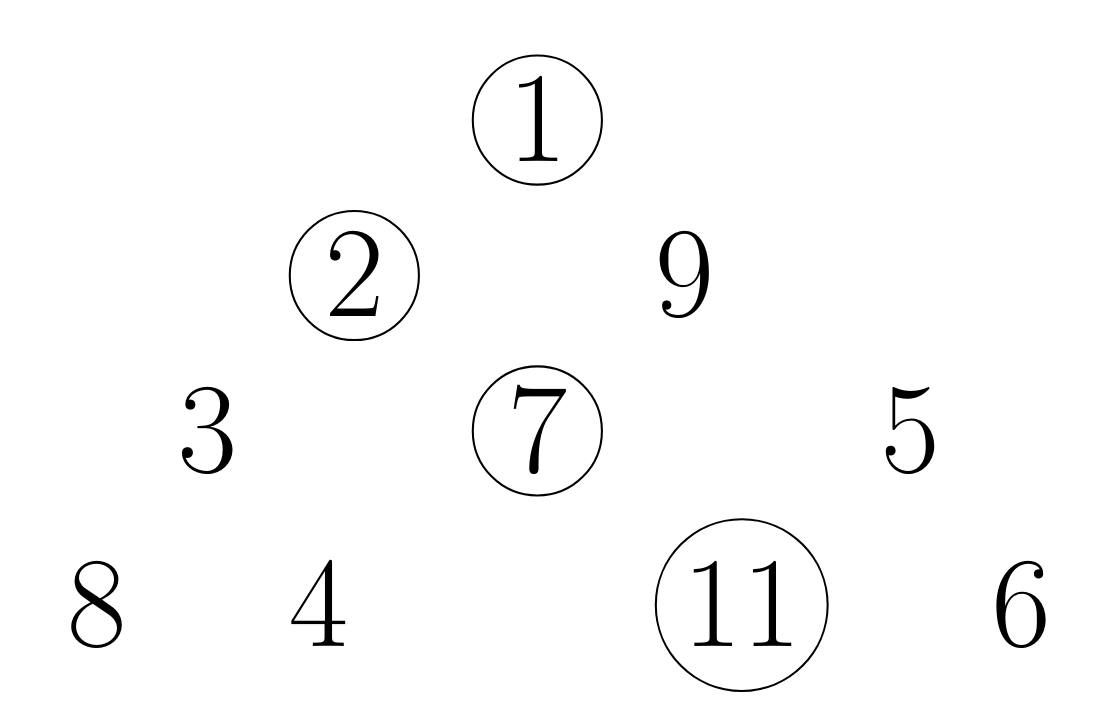
\includegraphics[scale=.15]{./img/discesa.png}}
    \small{\underline{\url{https://training.olinfo.it/\#/task/discesa/statement}}}
\end{frame}

\begin{frame}{Problemi}{Discesa massima}
    \begin{itemize}
        \item idee?
        \item quanti percorsi diversi esistono?
        \pause
        \begin{itemize}
            \item per $N$ volte devo scegliere se andare a dx o a sx
            \item ogni percorso \`e univocamente determinato dalla sequenza di scelte, quindi $2^N$ percorsi diversi
        \end{itemize}
        \pause
        \item i limiti su $N$ sono abbastanza piccoli da permetterci di eseguire una ricerca completa
    \end{itemize}
\end{frame}

\begin{frame}{Discesa massima}{}
    \makebox[\textwidth]{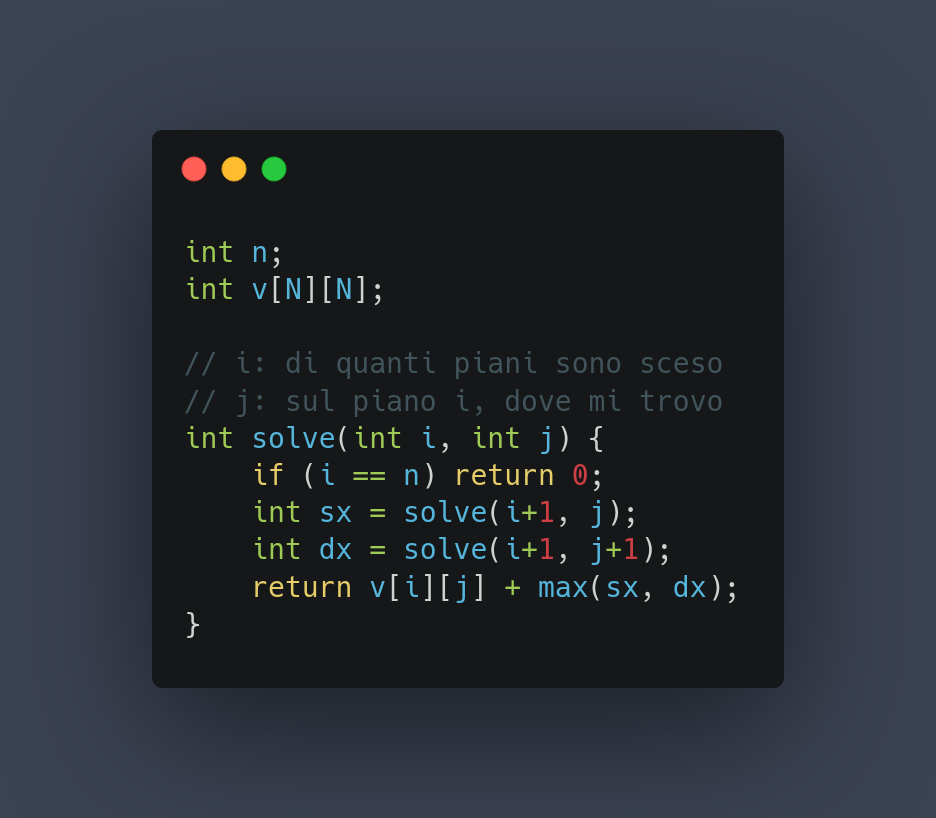
\includegraphics[scale=.30]{./img/discesa_rec.png}}
\end{frame}

\begin{frame}{Problemi}{Triangolo}
    \begin{exampleblock}{Triangolo}
        Stesso problema di prima, ma $N \leq 100$.
    \end{exampleblock}
    \pause
    Come si risolve?
    \pause
    \begin{itemize}
        \item memorizziamo la risposta per ogni stato
            \pause
            \begin{itemize}
                \item due chiamate a \texttt{solve(i, j)} ritornano lo stesso risultato
                \item possiamo calcolare ogni stato una sola volta
            \end{itemize}
        \item numero di stati: $O(N^2)$
        \item costo per transizione $O(1)$
        \item complessit\`a di tempo: $O(N^2 \cdot 1) = O(N^2)$
    \end{itemize}
    \small{\underline{\url{https://training.olinfo.it/\#/task/triangolo/statement}}}
\end{frame}

\begin{frame}{Triangolo}{}
    \makebox[\textwidth]{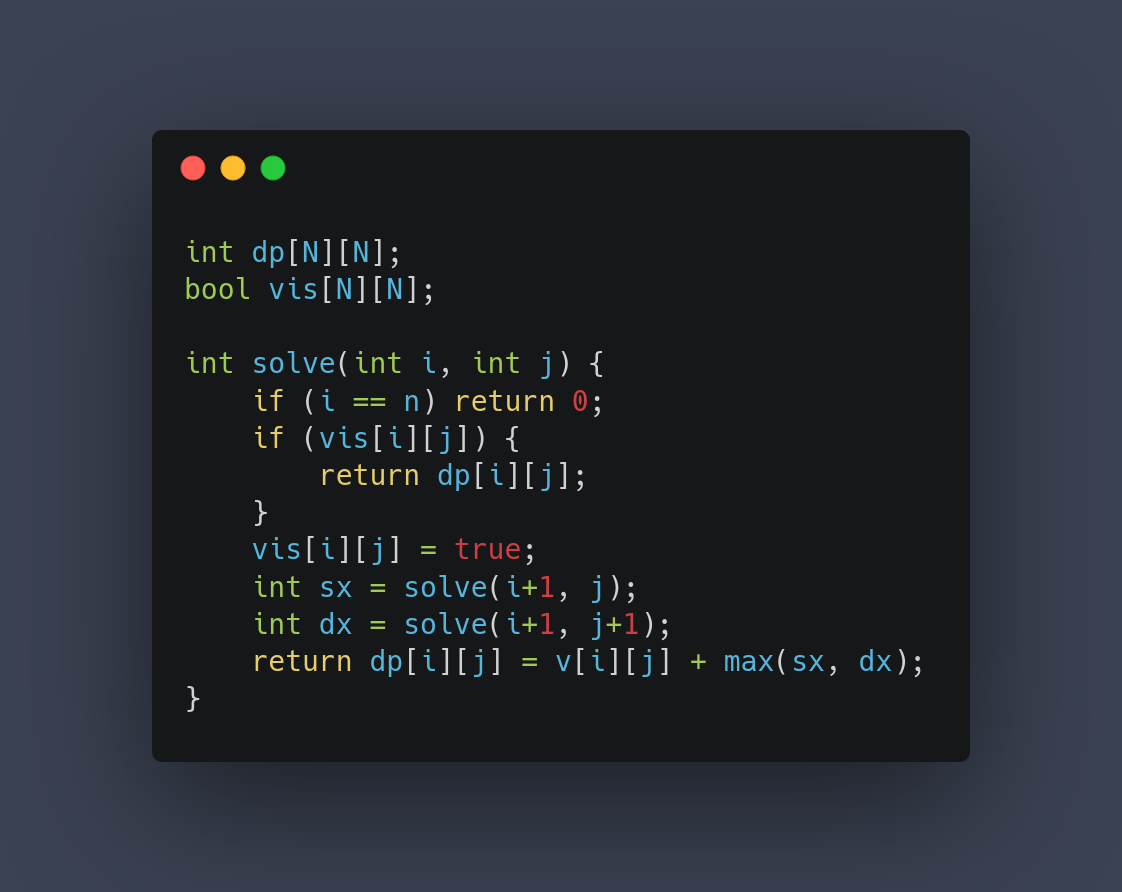
\includegraphics[scale=.25]{./img/triangolo.png}}
\end{frame}

\begin{frame}[fragile]{Problemi}{Grid paths}
    \begin{exampleblock}{Grid paths}
        Considera una griglia $N \times N$ con $N \leq 1000$ dove alcuni blocchi contengono delle trappole. Non \`e consentito camminare sulle trappole e puoi muoverti solo in basso o a destra. Calcola il numero di percorsi diversi dal quadratino in in alto a sinistra a quello in basso a destra. Stampa la risposta modulo $10^9 + 7$.
    \end{exampleblock}
    \small{\underline{\url{https://cses.fi/problemset/task/1638}}}
\end{frame}

\begin{frame}{Problemi}{Grid Paths}
    \begin{itemize}
        \item sia $dp[i][j]$ il numero di modi per andare da $(1;1)$ a $(i;j)$.
        \item per tutte le celle $(i;j)$ che non contengono trappole:
    \end{itemize}
    \pause
    \[
        dp[i][j] =
        \begin{cases}
            1 \quad &\text{se $(i;j) = (1;1)$} \\
            dp[i-1][j] + dp[i][j-1] \quad &\text{altrimenti}
        \end{cases}
    \]
\end{frame}

\section{Knapsack}
\begin{frame}{Knapsack}
    \begin{exampleblock}{Knapsack (o problema dello zaino)}
        Vengono dati $N \le 100$ oggetti, ognuno con un peso e un valore. Si vuole scegliere 
        un sottoinsieme di oggetti di valore massimo che abbia peso totale non superiore a $W \le 10^5$ (capacita dello zaino).
        $peso \le W$ e $valore \le 10^9$ per ogni oggetto.
    \end{exampleblock}
    \small{\underline{\url{https://atcoder.jp/contests/dp/tasks/dp_d}}}
\end{frame}

\begin{frame}{Knapsack}
    Cerchiamo di approcciare il problema anche con soluzioni non ottimali/errate. \\
    \begin{itemize}
        \item Potremmo provare tutti i sottoinsiemi di oggetti, ma \`e decisamente troppo lento (sono $O(2^N)$).\\
        \pause
        \item Potremmo ordinare gli oggetti per valore/peso decrescente e prendere i migliori fino a quando non superiamo la capacita dello zaino.\\
        \pause
        \begin{itemize}
            \item non \`e sempre ottimale! (es. $W=4$, $N=3$, $pesi = (1, 2, 2)$, $valori = (2, 3, 3)$).
        \end{itemize}
    \end{itemize}
\end{frame}

\begin{frame}{Knapsack}
    Semplifichiamo il problema: immaginiamo che gli oggetti ci arrivino uno alla volta.
    Possiamo scegliere se prendere l'oggetto o no (dobbiamo controllare di non superare $W$), quindi abbiamo 2 opzioni.\\
    \vfill
    \pause
    Rappresentiamo lo stato con 2 valori:
    \pause
    \begin{itemize}
        \item $pos$: l'indice dell'oggetto che stiamo considerando
        \item $peso$: il peso totale che abbiamo preso fino ad ora
    \end{itemize}
    \pause
    $dp[pos][peso]$ := valore massimo che possiamo ottenere conisderando gli oggetti da $0$ a $pos$ e avendo peso totale $peso$. La risposta \`e $\max(dp[N-1][j])$ per $j \leq W$.
    \pause
    \vfill
    Ci sono in totale $O(N \cdot W)$ stati, e per ognuno abbiamo 2 opzioni. La complessit\`a \`e $O(N \cdot W)$.\\
\end{frame}

\section{Longest Common Subsequence}
\begin{frame}{Longest Common Subsequence}{Problema}
    \begin{exampleblock}{LCS}
        Dati due stringhe $S$ e $T$ di lunghezza $N, M \le 3000$, calcola la lunghezza della sottosequenza piu lunga che sia presente sia in $S$ che in $T$.
    \end{exampleblock}
    \small{\underline{\url{https://atcoder.jp/contests/dp/tasks/dp_f}}}
\end{frame}

\begin{frame}{Longest Common Subsequence}{Soluzione}
    $dp[i][j]$ := lunghezza della LCS tra $S[i\dots N]$ e $T[j\dots M]$. \\
    La risposta \`e $dp[0][0]$.
    \vfill
    \pause
    Ci troviamo in $dp[i][j]$. Abbiamo due casi possibili:
    \begin{itemize}
        \item $S[i] \ne T[j]$, allora $dp[i][j] = max(dp[i+1][j], dp[i][j+1])$;
        \item $S[i] = T[j]$, allora $dp[i][j] = 1 + dp[i+1][j+1]$.
    \end{itemize}
    \pause
    \vfill
    Il numero di stati \`e $O(N \cdot M)$, e per ogni stato abbiamo 2 opzioni, quindi la complessit\`a \`e $O(N \cdot M)$.\\
    \pause
\end{frame}

\begin{frame}{Problemi addizionali}
    \underline{\url{https://training.olinfo.it/\#/task/ois_nonna/statement}}
    \underline{\url{https://training.olinfo.it/\#/task/ois_police3/statement}}
    \underline{\url{https://training.olinfo.it/\#/task/ois_police4/statement}}
    \underline{\url{https://training.olinfo.it/\#/task/lotteria/statement}}
    \underline{\url{https://cses.fi/problemset/}}
    \underline{\url{https://atcoder.jp/contests/dp/tasks}}
\end{frame}

\end{document}
